% ------------------------------------------------------------------------
% file `main-bookexercise-5-solution-body.tex'
%
%     solution of type `bookexercise' with id `5'
%
% generated by the `exerciseanswer' environment of the
%   `xsim' package v0.21 (2022/02/12)
% from source `main' on 2026/10/17 on line 2380
% ------------------------------------------------------------------------
1. 正确。\\

2. 正确。\\

3. 选B。A、C、D均存在平衡因子的绝对值大于1的节点，如图所示。\\
\begin{center}
    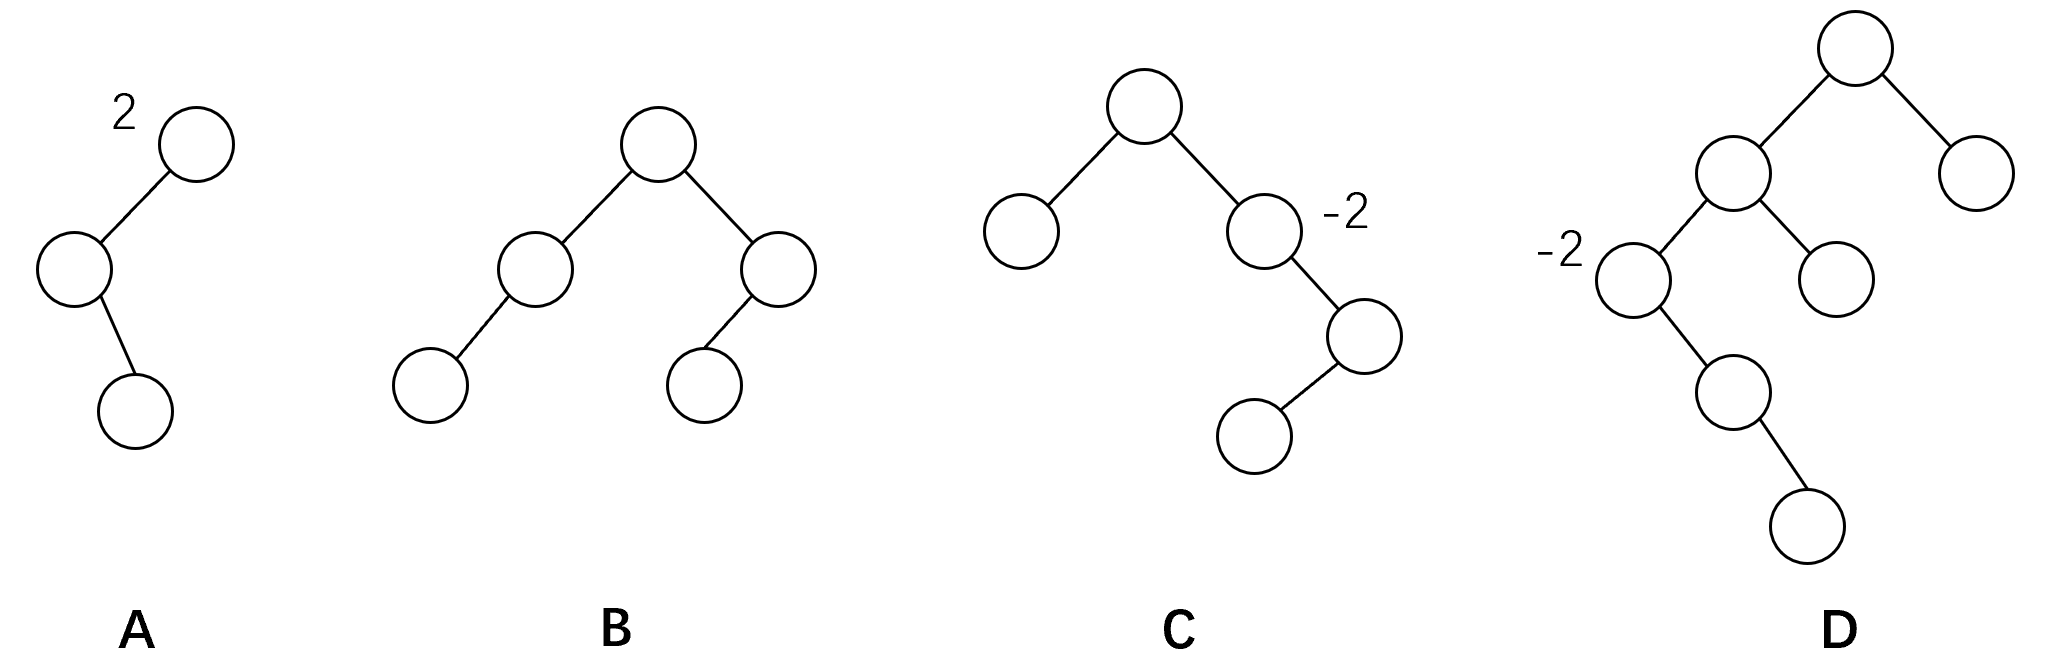
\includegraphics[width=0.80\textwidth]{assets/pics_and_ppts/ch4/09408_平衡二叉树定义答案图.png}
\end{center}

4. 选A。各选项查找过程如下图所示：
\begin{center}
    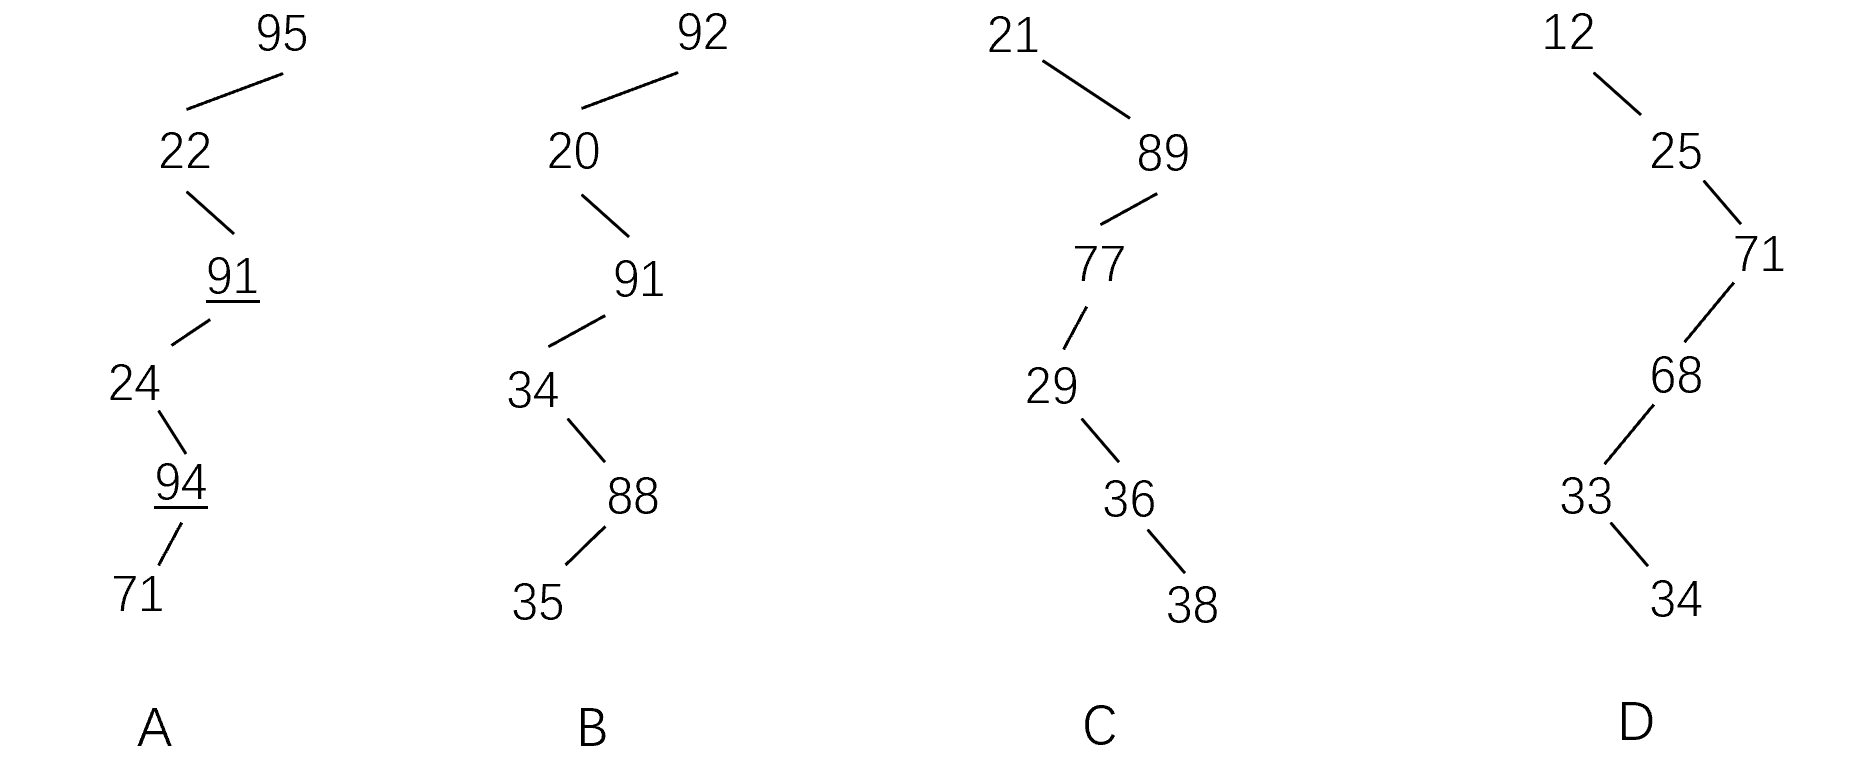
\includegraphics[width=0.8\textwidth]{assets/pics_and_ppts/ch4/11408_二叉查找树查找路径答案图.png}
\end{center}
图A，91的左子树出现了94，大于91，因此不可能是二叉排序树的查找路径。    \\

5. 选C。插入48后，据新插入节点48最近的失衡节点为24（根节点），平衡因子为1-3=-2，为RL型失衡。先对53右旋，再对24左旋，调整后37的左、右孩子分别是24、53，如下图所示。
\begin{center}
    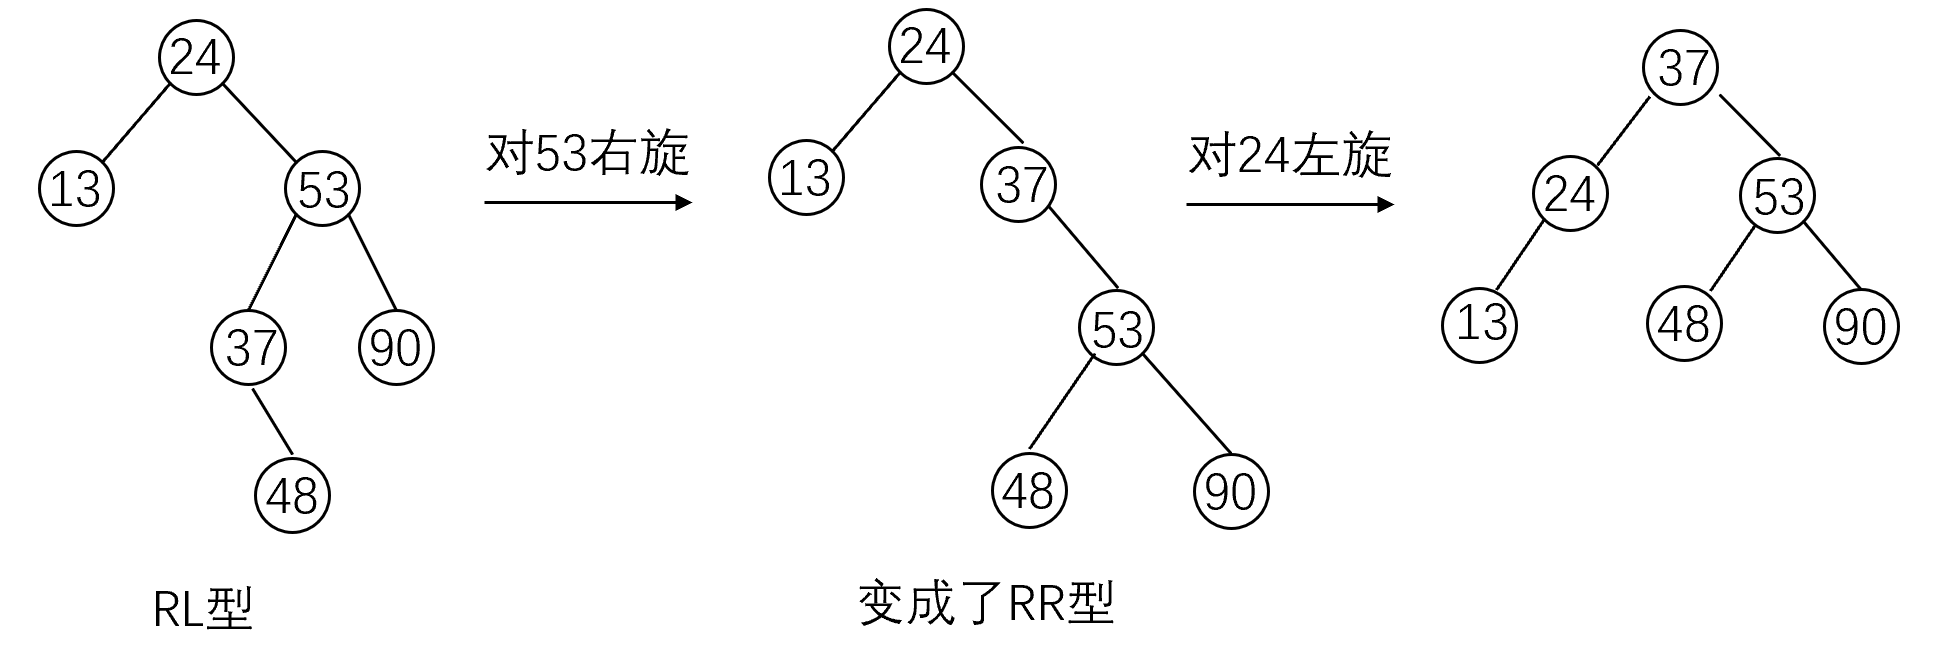
\includegraphics[width=0.81\textwidth]{assets/pics_and_ppts/ch4/10408_平衡二叉树插入后37的左右孩子值答案图.png}
\end{center}

\vspace{\baselineskip}

6. 选B。B项插入序列生成的二叉排序树如图所示：
\begin{center}
    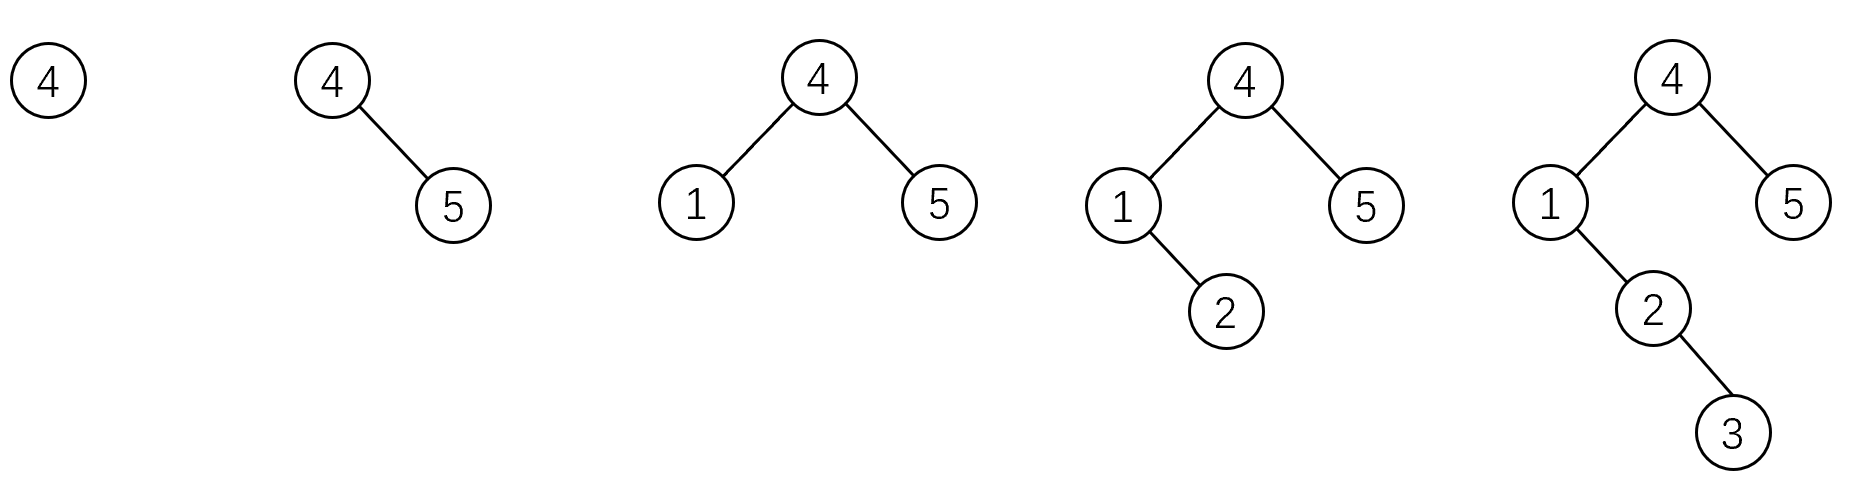
\includegraphics[width=0.78\textwidth]{assets/pics_and_ppts/ch4/20408哪一个序列不能生成图示二叉排序树答案图.png}
\end{center}

\vspace{\baselineskip}

7. 我们从根节点开始，向左右子树寻找两个目标节点。如果发现左边找到了一个、右边也找到了一个，那么当前节点一定是它们的最近公共祖先。完整代码如下：
\begin{cppcode}
    node* LowestCommonAncestor(node* root, int a, int b) {
        if( root == NULL ) return NULL;

        if( root == p || root == q ) return root;

        node* left = lowestCommonAncestor(root->left, p, q);
        node* right = lowestCommonAncestor(root->right, p, q);
        if( left != NULL && right != NULL ) return root;
        if( left ) return left;
        if( right ) return right;

        return NULL;

    }
\end{cppcode}
寻找公共祖先的代码是极难理解的。别急，我和大家一起慢慢将其拆解。建议大家结合下面的代码注释以及图中所示例子的查找过程共同来理解。
首先我们从根节点开始，向左右子树寻找两个目标节点。如果
发现左边找到了一个、右边也找到了一个，那么当前节点一定是它们的最近公共祖先：
\begin{cppcode}

    node* left = LowestCommonAncestor(root->lchild, 4, 5);
    node* right = LowestCommonAncestor(root->rchild, 4, 5);

    if (left != NULL && right != NULL)
        return root;
\end{cppcode}
如果沿途找到了某NULL节点，说明此条路径上没有有意义的信息，直接返回NULL；

若找到了某待查关键字，或两个关键字的公共祖先之后，则将相应指针沿路径向上返回：
\begin{cppcode}
// 沿路径查找到了NULL，说明该路径上不存在有用的信息。
    if( root == NULL ) return NULL;

    node* left = LowestCommonAncestor(root->lchild, 4, 5);
    node* right = LowestCommonAncestor(root->rchild, 4, 5);

// 若找到了某待查关键字，将该节点指针向上返回
    if( root == p || root == q ) return root;

// 这种情况成立，则一定是left和right分别是待查找的两个关键字的指针。此时root就是公共祖先，向上返回，一直传递上去。
    if (left != NULL && right != NULL)
        return root;

    // 此前（更下层的递归中）存在有用的信息（左子树中有待查关键字，或已经在左子树中找到了最近公共祖先），将该有用的信息向上返回，传递上去
    if(left) return left;
    // 此前（更下层的递归中）存在有用的信息（右子树中有待查关键字，或已经在右子树中找到了最近公共祖先），将该有用的信息向上返回，传递上去
    if(right) return right;

    // 若左右子树都不存在有用的信息，返回NULL，表示这条路径上没有有用的信息。
    return NULL;
\end{cppcode}
left、right实际上有两层含义：

第一层：未找到公共祖先时，left或right表示该节点左（右）子树中待查找的关键字的指针。（第一种有用的信息）

第二层：找到公共祖先后，left及right的含义就是该节点的左（右）子树中是否存在要找的公共祖先节点，若存在，left或right表示的就是公共祖先节
点的指针，若不存在，left或right为NULL。（第二种有用的信息）\\[0.3em]


我们给出在下图所示的二叉树中，寻找4和5的公共祖先的过程。
\begin{center}
    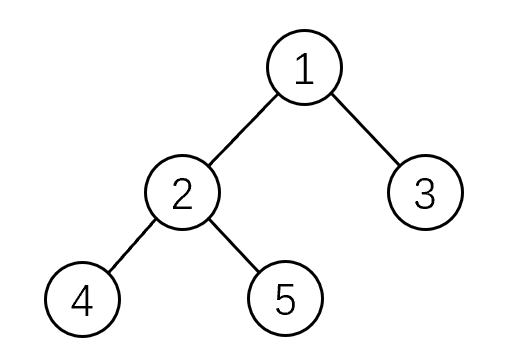
\includegraphics[width=0.25\textwidth]{assets/pics_and_ppts/ch4/习题_寻找公共祖先答案图.png}
\end{center}

第一步，当前节点root是 1，它既不是 4，也不是 5。
因此，算法继续向下查找：\\
- 左子树：从节点 2 开始。\\
- 右子树：从节点 3 开始。\\

第二步：进入节点 2，
节点 2 又会向左右子树查找：\\
- 左边进入节点 4。\\
- 右边进入节点 5。

当递归来到节点 4 时，发现它就是目标节点，于是直接返回节点 4。
同理，来到节点 5 时，直接返回节点 5。
于是，节点 2 这一层得到：
\begin{center}
    node* left = LowestCommonAncestor(root->lchild, 4, 5);       // left是节点4的指针 \\
    node* right = LowestCommonAncestor(root->rchild, 4, 5);     // right是节点5的指针
\end{center}
两边都不为空！说明两个目标节点分别出现在节点 2 的左右子树中。
因此，返回节点 2。\\

第三步：返回节点 1，
节点 2的递归函数中 返回了节点 2，意味着节点 1 的左侧查找结果是节点 2。
而节点 3 的子树里没有 4 或 5，所以右侧返回 nullptr。
因此，节点 1 得到：
\begin{center}
    node* left = LowestCommonAncestor(root->lchild, 4, 5);       // left是节点2的指针 \\
    node* right = LowestCommonAncestor(root->rchild, 4, 5);     // right是NULL
\end{center}
因为只有左边有结果，节点 1的递归函数栈中 就把左边的结果（节点2的指针）继续返回。
得到最终答案是节点 2。



